% Created:  Wed 09 Jul 2014 03:00 PM
% Modified: Wed 09 Jul 2014 03:00 PM
% @author Josh Wainwright
% File name : clusters.tex

\part{Cluster Analysis}
\label{prt:cluster_analysis}

Cluster analysis is the grouping of a set of objects or items in a spatially or
informationally logical way such that the items that are placed in the same
group are more similar to each other than they are to the objects in the other
groups in the set. These groups shall be called \emph{clusters}. When dealing
with images, the clustering that is of interest is based on spatial location,
i.e., clusters should be composed of objects that are close together in the
image and clusters should be separated by regions of emptiness or background
level noise.

One of the primary reasons for chosing the quadtree method over the simple grid
methods was that the simple act of placing the objects, in this case
coordinates of data points, into the quadtree starts the process of analysing
the data. Since the points end up in a tree structure with the number of points
closely separated being on the lowest levels of the tree, the data is already
clustered in a way.

There are a number of alternative methods of identifying clusters in images.

% Created:  Mon 30 Jun 2014 05:32 PM
% Modified: Thu 31 Jul 2014 10:16 AM
% @author Josh Wainwright
% File name : rolling-ball.tex

\section{Rolling Ball Analysis}
\label{sec:rolling_ball_analysis}

The accessible surface area (ASA) algorithm, also known as the ``Rolling Ball
Method'', is a technique used in image processing for describing the outer
limit of a cluster of points. It is derived from biological molecules analysis
where it describes the surface area of a molecule that is accessible to a
solvent.

The rolling ball method can be used to analyse a cluster of points by imagining
a solid ball that sits against one of the outer-most points. From here it is
``rolled'' around the cluster such that it is always touching at least one
point. Once the ball has reached the point it started at, the line that the ball
traced is reduced in size by the radius of the ball. This line then represents
the outer limit of the cluster.

The size of the ball must be chosen depending on the average separation of the
points within the cluster.

\begin{figure}[tbhp]
	\centering
	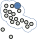
\includegraphics[width=4.2cm]{rolling-ball.pdf}
	\caption{The rolling ball method for cluster detection provides a way of
		identifying clusters, as inspired by molecular biology. A very simple
		implementation can be fast but is not particularly successful at
		finding clusters unless the data points are very dense and there is no
		noise.} \label{fig:rolling-ball}
\end{figure}

A simple approximation of this technique can be acheived by using the same
\texttt{open}-ing and \texttt{close}-ing processes as are described in
Section~\ref{sec:simple_grid_method}.

% Created:  Thu 10 Jul 2014 04:22 PM
% Modified: Thu 10 Jul 2014 04:22 PM
% @author Josh Wainwright
% File name : quadtree-traversal.tex

\section{Quadtree Traversal}
\label{sec:quadtree_traversal}

Whether the quadtree is stored in memory as a recursive quadtree data
structure, or as hash table, Section~\ref{sub:hash_table_implementation}, the
most important and computationally intensive step is extracting the clusters at
the correct depth and disregarding those data points that can be attributed to
noise.

The quadtree numbering system chosen lends itself very well to analysis based
on spatial location and the proximity of neighbours to a given cell being
examined. The neighbours of interest, named as \emph{rook's case} neighbours
% TODO Add abel and mark paper reference.
by~ref{}, are the four cells that lie to the north, east, sound and west of the
current

\begin{figure}[tbhp]
	\centering
	\includegraphics[width=0.88\linewidth]{propogation.pdf}
	% TODO caption
	\caption{Propagation}
	\label{fig:propogation}
\end{figure}

When discovering clusters via this propagation technique, care must be taken to
avoid a run-away situation where every node in the tree gets included. This
would happen when looking at the neighbours of a node and blindly including
them. Since every internal node has exactly four neighbours, the propagation
would terminate only when reaching the edge nodes.

Instead, the depth of the node must be considered. Again, the simplest method
is not sufficient. If the propagation is limited to a given node depth, even if
this is not the same as the deepest node, the size of any clusters that are
identified will be limited, as shown in Figure~\ref{fig:propogation-halting}.
Since the depth to consider is not able to change, when the neighbours of the
blue cell are checked, no correct neighbours are found and so the process
terminates. When able to view the larger structure of the cells, however, it is
clear that the structure continues beyond the gap.

\begin{figure}[tbhp]
	\centering
	\includegraphics[width=0.7\linewidth]{propogation-halting.pdf}
	\caption{propogation-Halting}
	\label{fig:propogation-halting}
\end{figure}

To avoid this, a certain amount of leniency must be given when deciding what
constitutes a neighbour. Given an appropriate value, this would allow both of
the larger white cells in Figure~\ref{fig:propogation-halting} to be included.

The \emph{depth range} shall define the levels that are to be considered when
choosing neighbours with respect to a target depth. Since clusters are being
considered areas of increased density of points, all cells with a depth greater
than the target depth shall be allowed, so the purple cells in
Figure~\ref{fig:propogation-halting} would be included when the target depth is
the same as the depth of the included red cells. A depth range of zero is
eqivalent to the situation above where only cells of a given depth are
considered. A depth range of 1 would mean that the white square in
Figure~\ref{fig:propogation-levels}\,b) would be included but not in~c),
whereas a depth range of three would include both.

\begin{figure}[tbhp]
	\centering
	\includegraphics[width=0.88\linewidth]{propogation-levels.pdf}
	\caption{propogation-Levels}
	\label{fig:propogation-levels}
\end{figure}

